\chapter{Results}
\label{chapter:results}
We use two distinct approaches to compute the parameter that specify the function of \acfp{DNMT}, especially their binding and methylation probabilities. In our computer simulation we focus on DNMT1 and DNMT3. The enzyme activity is modelled using a \acf{HMM}, that stores the binding state of all methyltransferases and the methylation state for each (\acf{CpG})-position. Three scenarios are considered: DNMT1 \acf{KO}, where only DNMT3 is active; DNMT3a/b \ac{KO}, where DNMT3 is absent and \acf{WT}, where both enzymes are involved in the methylation process. For \ac{WT} it is assumed the order of enzyme activity is DNMT1 on daughter strand, DNMT3 on daughter strand and DNMT3 on parental strand. Supposing the DNA is not unmethylated before replication, an initial methylation pattern is given by \ac{WT} data. Thereupon, the iterations of the simulation generate a methylation pattern distribution that is compared to a measured distribution in order to evaluate it.\newline
The measured datasets are derived using hairpin-bisulfite sequencing. Three loci are considered; two repetitive elements: major Satellites (mSat) and IAPLTR1, LTR-retrotransposons (IAP) and an alpha feto protein gene (Afp). For more details see \cite{Wolf}.

\section{Maximum Likelihood Estimation}
\label{MLE}
\begin{figure}[h]
\begin{center}
\begin{tabularx}{\textwidth}{l|c|c|c|c|c|c}
locus&	restrictions&	$\rho$&	$\tau$&	$\mu$&	$\delta$&	likelihood\\
\hline
mSat&	&	0.894&	0.276&	0.782&	1&	4757\\%*
mSat&	$\rho=1$&	1&	0.275&	0.565&	1&	4704\\%**
mSat&	$\tau=1$&	$\approx1$&	1&	0.17&	0.279&	4713\\
Afp&	&	1&	0&	0.809&	0.857&	1692\\%X
Afp&	$\delta=1$&	$\approx1$&	0.219&	0.491&	1&	963\\%**
Afp&	$\delta=1 \wedge \mu=1$&	1&	0.124&	1&	1&	1078\\%**
IAP&	&	0&	0&	0.028&	0.566&	2675\\
IAP&	$\rho=1$&	1&	0.974&	0.267&	0.198&	1614\\
IAP&	$\tau=1$&	0.869&	1&	0.265&	0.189&	1579\\
\end{tabularx}
\end{center}
\label{DNMT1KO}
\caption{Parameter for minimal negative log-likelihoods of three loci for DNMT1KO.}
\end{figure}

\begin{figure}[h]
\begin{center}
\begin{tabularx}{\textwidth}{l|c|c|c|c|c|c}
locus&	restrictions&	$\rho$&	$\tau$&	$\mu$&	$\delta$&	likelihood\\
\hline
mSat&	&	0.234&	1&	0.736&	0.426&	3496\\%*
mSat&	$0.8 \leq \mu \leq 1$&	$\approx 0$&	$\approx 1$&	0.8&	0.443&	3430\\%**
mSat&	$\rho=1$&	1&	0.929&	0.885&	0.417&	3429\\%**
Afp&	&	$\approx 0$&	0.488&	0.366&	$\approx 0$&	2659\\%*
Afp&	$\mu=1$&	0.773&	0.709&	1&	0.448&	1091\\%**
Afp&	$0.8 \leq \mu \leq 1$& 0.51&	0.866&	0.8&	0.267&	1046\\
IAP&	&	$\approx 0$&	0.994&	0.837&	0.496&	2494\\%*
IAP&	$\rho=1$&	1&	0.901&	$\approx1$&	0.391&	2423\\%**
IAP&	$\mu=1$&	0.974&	0.901&	0.892&	0.375&	2456\\%**
\end{tabularx}
\end{center}
\label{DNMT3KO}
\caption{Parameter for minimal negative log-likelihoods of three loci for DNMT3a/bKO.}
\end{figure}

\subsection{mSat}
\label{mSat}
In the first method, the program parameters were estimated using the likelihood function from chapter \ref{Maximum Likelihood Estimation}. First, the locus mSat will be considered here as it is the one with the fewest \acp{CpG}. Let us focus on the \ac{KO} data first, where either DNMT1 or DNMT3 are active. Looking at the first row of table \ref{DNMT1KO} and \ref{DNMT3KO}, where the results of \acf{MLE} are displayed for locus mSat and DNMT3 and DNMT1 respectively, one can see the differences in the function of the two enzymes as their parameters are clearly distinguishable. Where the association probability is very high and the disassociation probability rather low for DNMT1, the values are vice versa for DNMT3. This means that DNMT1 will always bind to the DNA and the few times where it falls off, it is very likely that it will bind again.\newline
Where the association length, the number of \acfp{bp} where an enzyme is bound, is very high for DNMT1, the same length is small for DNMT3. DNMT3 is not very likely to bind to the DNA and will fall off after a short wile. Moreover, the de novo methylation probability is higher for DNMT3, which is consistent with our suggestions. Whereas the maintenance methylation probability is between 0.7 and 0.8 for both enzymes, DNMT1 will perform more maintenance methylation than DNMT3 because its association length is higher. If we multiply the maintenance methylation probability of DNMT3, $\mu_3$, with its association probability, we get the real value of $\mu_3$ because the enzyme needs to be bound to methylate. $\mu_3 \times \tau_3$ is equal to 0.216 and thus clearly smaller than the maintenance methylation probability of DNMT1.
\begin{figure}[h]
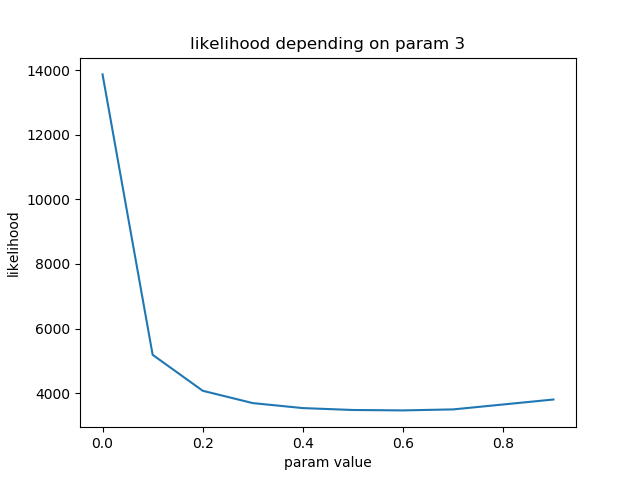
\includegraphics[scale=0.7]{../likelihoodPlot3DNMT3KO.png}
\label{rangedelta}
\caption{Negative log-likelihood depending on parameter $\delta$; the other three parameter values are fixed.}
\end{figure}

%mSat restrictions
We evaluate the likelihood function further by investigating the borders of the function. We thus compare the value of the likelihood after each parameter was set to zero and one to the present minimum. Further, during the \ac{MLE} computation, it was striking that sometimes some parameters were difficult to identify because the range where this parameter maximizes the likelihood was wide as visible in figure \ref{rangedelta}. Therefore, another approach was to fix an interval for the parameters, which may maximize the likelihood. The best results for the parameter restrictions for mSat are shown in row two and three in table \ref{DNMT1KO} and \ref{DNMT3KO}.\newline
For both methyltransferases, the likelihood is maximized by setting $\rho$ to one. $\tau$ and $\delta$ do not change significantly compared to the result without parameter restriction for DNMT3, while $\mu$ decreases by 0.217.\newline
For DNMT1 $\tau$ decreases and $\mu$ increases a bit such that all parameters besides $\delta$ are very high. Regularly, the interpretation of a high $\rho$ would be that the enzyme falls off at each \ac{bp}, but in this case, if $\tau$ is next to one too, the \ac{DNMT} will immediately bind again. In this model, the enzyme can be interpreted as very processive. We are not able to distinguish between a low disassociation probability and a very high dis- and reassociation probability as both combinations lead to the event that the methyltransferase is bound to one \ac{bp} and its successor. Thus, DNMT1 is interpreted as very processive and the result with $\rho=1$ and $\tau \approx 1$ is similar to the previous result.\newline
Another very likely scenario for DNMT3 is, if $\tau$ was set to one. Then $\rho$ is approximately one, but the methylation probabilities decrease compared to the approach without parameter restriction. The interpreting is different here, because the methylation activity is low. DNMT3 seems to work processive in this case but methylation events occur rather rarely.\newline
In the third scenario of DNMT1 and locus mSat, $\mu$ was restricted to the interval [0.8,1]. Compared to row one of table \ref{DNMT3KO}, both parameter estimations are very similar again; only the disassociation probability is even lower. Both results suggest a processive behaviour of DNMT1 with high methylation probabilities.\newline
In sum...

\subsection{Afp}
\label{Afp}

\subsection{IAP}
\label{IAP}

\subsection{WT}
\label{WT}
\begin{figure}[h]
\begin{center}
\begin{tabularx}{\textwidth}{l|c|c|c|c|c|c}
locus&	restrictions&	$\rho$&	$\tau$&	$\mu$&	$\delta$&	likelihood\\
\hline
mSat&	&	0.56&	0.872&	$\approx1$&	0.472&	3430\\
	&	&	0&	$\approx1$&	0.051&	0.572&	\\
\hline
Afp&	&	0.026&	0.96&	0.888&	$\approx1$&	1110\\
	&	&	0.419&	0.371&	0.797&	0.914&	\\
\hline
Afp&	$0 \leq \delta1 \leq 0.3$&	0.301&	0.895&	1&	0.18&	1077\\%**
	&	&	0.988&	0.858&	$\approx0$&	$\approx1$&	\\
\hline
Afp&	$0 \leq \delta1 \leq 0.5 \wedge 0.8 \leq \delta3 \leq 1$&	0.379&	0.915&	$\approx1$&	0.5&	1056\\
	&	&	0.268&	0.754&	$\approx0$&	0.956&	\\
\hline
IAP&	&	0.416&	0.927&	0.963&	0.749&	1838\\%*
	&	&	0.708&	0.912&	0&	0.61&	\\
\hline
IAP&	$0 \leq \delta1 \leq 0.5$&	0.17&	0.876&	0.957&	$\approx0$&	1832\\%**
	&	&	0.575&	0.879&	$\approx0$&	$\approx1$&	\\
\end{tabularx}
\end{center}
\label{WT33}
\caption{Parameter for minimal negative log-likelihoods of three loci for WT after 33 cell divisions, the first row for every locus shows the parameter for DNMT1($\rho1, \tau1, \mu1, \delta1$); the second row for DNMT3($\rho3, \tau3, \mu3, \delta3$).}
\end{figure}

\begin{figure}[h]
\begin{center}
\begin{tabularx}{\textwidth}{l|c|c|c|c|c|c}
locus&	restrictions&	$\rho$&	$\tau$&	$\mu$&	$\delta$&	likelihood\\
\hline
mSat&	&	1&	0.907&	1&	0.701&	3660\\%X
	&	&	1&	0.053&	0&	0&	\\
\hline
mSat&	$0 \leq \rho1 \leq 0.2 \wedge 0.4 \leq \rho3 \leq 1$&	0.2&	1&	0.89&	0.284&	3449\\%**
	&	$\wedge 0.5 \leq \delta3 \leq 1$&	1&	0.584&	0.286&	0.694&	\\
\hline
Afp&	&	$\approx0$&	0.916&	0.87&	$\approx0$&	3510\\
	&	&	0.971&	0.963&	0.399&	0.748&	\\
\end{tabularx}
\end{center}
\label{WT33}
\caption{Parameter for minimal negative log-likelihoods of three loci for WT after 100 cell divisions, the first row for every locus shows the parameter for DNMT1($\rho1, \tau1, \mu1, \delta1$); the second row for DNMT3($\rho3, \tau3, \mu3, \delta3$).}
\end{figure}

\section{Approximative Bayesian Computation}
\label{ABC}